\chapter{\IfLanguageName{dutch}{Stand van zaken}{State of the art}}
\label{ch:stand-van-zaken}

% Tip: Begin elk hoofdstuk met een paragraaf inleiding die beschrijft hoe
% dit hoofdstuk past binnen het geheel van de bachelorproef. Geef in het
% bijzonder aan wat de link is met het vorige en volgende hoofdstuk.

% Pas na deze inleidende paragraaf komt de eerste sectiehoofding.
Dit overzicht biedt inzicht in de huidige stand van zaken en vormt de basis voor een weloverwogen keuze bij de ontwikkeling van een Proof of Concept (PoC). Dit betreft zowel de technische als de juridische aspecten. Daarnaast wordt in dit deel ook stilgestaan bij het belang van een vlot supportproces binnen IT.

Concreet komen de volgende onderwerpen aan bod:
\begin{itemize}
    \item \textbf{IT-support chatbot} - Wat zijn de mogelijkheden van om een IT-support chatbot te maken aan de hand van een LLM en welke factoren moeten in overweging worden genomen?
    \item \textbf{De AI Act en de belangrijkste richtlijnen} - Een overzicht van de relevante wet- en regelgeving en de impact hiervan op RAG-toepassingen.
    \item \textbf{Best practices voor IT-supportprocessen} - Inzichten in hoe RAG kan worden toegepast binnen IT-support en welke methodologieën het best kunnen worden gevolgd.
\end{itemize}

\section{IT-support chatbot}
    
    Om een IT-support chatbot te ontwikkelen, moeten verschillende aspecten in overweging worden genomen. Bij het gebruik van een LLM-model zijn er twee belangrijke opties: Retrieval-Augmented Generation (RAG) en Cache-Augmented Generation (CAG). Beide methoden maken gebruik van een LLM en verrijken de kennis van dit model met behulp van eigen documenten. Echter, beide benaderingen hebben specifieke voor- en nadelen. Het is daarom essentieel om deze zorgvuldig af te wegen om een weloverwogen keuze te maken voor een Proof of Concept (PoC).
    
    \subsection{Retrieval Augmented Generation}
    
    \textit{Large Language Models} (LLM) hebben de afgelopen jaren een enorme opmars gemaakt en vandaag de dag hebben deze modellen een brede impact op verschillende domeinen in de samenleving. Ondanks hun indrukwekkende mogelijkheden brengen LLM’s ook enkele nadelen met zich mee. Zo kunnen ze hallucineren, beschikken ze niet altijd over de meest actuele informatie, en missen ze vaak domein- en bedrijfsspecifieke kennis.  
    
    Een mogelijke oplossing voor deze beperkingen is \textit{Retrieval-Augmented Generation} (RAG). Deze techniek combineert de kracht van LLM’s met externe databronnen om nauwkeurigere en beter onderbouwde antwoorden te genereren. In deze sectie wordt toegelicht wat RAG is, hoe het werkt en op welke manier het kan bijdragen aan de ontwikkeling van een effectieve support chatbot.
    
    \subsubsection{Wat is RAG}
    RAG, oftewel Retrieval-Augmented Generation, is een techniek die, zoals eerder vermeld, een oplossing biedt voor de tekortkomingen van klassieke LLM’s. Door externe databronnen te gebruiken, kan een traditioneel LLM-model betere resultaten behalen. Deze methode maakt het mogelijk om domeinspecifieke data te integreren en modellen bij te werken met actuele informatie. Zo kunnen klassieke LLM’s worden verrijkt met nieuwe, up-to-date gegevens die voldoen aan specifieke behoeften \autocite{Wu2024}.
    
    Om RAG in de praktijk toe te passen, moeten een aantal stappen worden doorlopen. Deze worden in het volgende deel nader toegelicht, maar samengevat bestaat het proces uit de volgende fasen:
    
    \begin{enumerate}
        \item {Ophalen}
        \item {Verrijking}
        \item {Generatie}
    \end{enumerate}
    
    \subsubsection{Hoe werkt RAG}
    
    Het doel van RAG is om een LLM te verrijken met specifieke kennis, zodat de gebruiker beter ondersteund wordt bij het beantwoorden van gerichte vragen. Dit proces bestaat uit drie hoofdfasen. Eerst wordt relevante informatie opgehaald (Retrieval). Vervolgens wordt het antwoord verrijkt op basis van de beschikbare documentatie. Tot slot genereert de LLM een antwoord op de gestelde vraag.
    
    Op Figuur \ref{fig:Rag process} is te zien die dit proces illustreert.
    
    \begin{figure}[H]
        \centering
        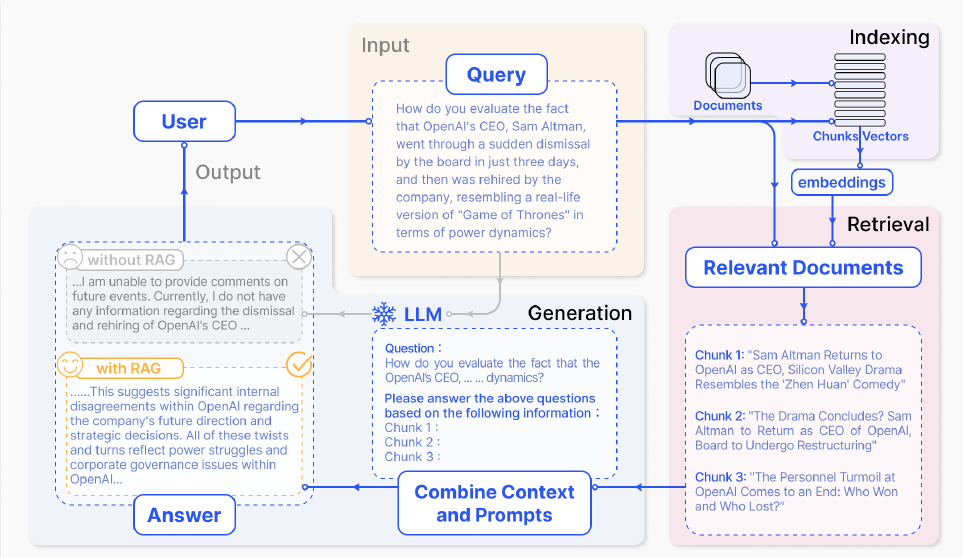
\includegraphics[width=\textwidth]{RagGao2023.png}
        \caption{Een generieke RAG architectuur \cite{Gao2023}}
        \label{fig:Rag process}
    \end{figure}
    
    \paragraph{Ophalen}
   
    
    %TODO laten corrigeren gramaticaal en de delen die hierin worden besproken verder uitbreiden met meer tekst zdat het langer is dan 2 zinnen.
    % gebruik figuur 2 van Wu2024 om te illustreren
    Voordat de LLM kan worden ondervraagd met de informatie die we via documentverrijking in het model stoppen, is er eerst veel voorbereidend werk nodig. Het proces houdt in dat relevante documenten, samen met de gestelde vraag, via een vector database worden geïnjecteerd in de LLM om tot een passend antwoord te komen. Hiervoor moeten verschillende stappen worden doorlopen.
    
    Allereerst moet er een selectie worden gemaakt van de relevante documenten, die vervolgens worden opgedeeld in kleinere delen, ook wel “chunks” genoemd, zoals vaak in de vakliteratuur wordt aangeduid. Dit wordt voornamelijk gedaan omdat sommige documenten te lang zijn om op een efficiënte manier verwerkt te worden. Daarnaast helpen chunks bij het ophalen van gerichte informatie uit de vector database. 
    
    Er kunnen verschillende technieken worden toegepast om documenten in chunks te verdelen. Een mogelijkheid is om te werken met een vaste lengte of een vast aantal tokens, zodat elke chunk een gelijke lengte heeft. Een andere optie is om, wanneer het om tekstdocumenten gaat, te werken met chunks op basis van een bepaald aantal zinnen. Dit heeft als voordeel dat de semantiek van een chunk beter behouden blijft dan wanneer er wordt gewerkt met chunks van vaste lengte \autocite{Wang2024}.

    Het uiteindelijke doel is om de chunks te vertalen naar embeddings, die vervolgens in een vector database worden opgeslagen. Een embedding is de vectorrepresentatie van een chunk. Deze embeddings worden opgeslagen in een vector database \autocite{Wu2024}, die speciaal is ontworpen voor het opslaan en efficiënt ophalen van embeddings. Het proces wordt weergegeven in de onderstaande figuur.
   
     \begin{figure}[H]
        \centering
        \includegraphics[width=\textwidth]{retrieverWu2024.png}
        \caption{Documentverwerking en opslag in een vector database via embeddings \cite{Wu2024}}
        \label{fig:RAG opmaken vector database}
    \end{figure}
    
    Zodra de documenten via embeddings zijn toegevoegd aan de vector database, zal een gebruiker in de context van RAG (Retrieval-Augmented Generation) ook vragen stellen. Een vraag of query wordt, net als de documenten, vertaald naar embeddings. Op basis van deze embeddings worden de top-k dichtstbijzijnde buren uit de vector database opgehaald. Dit betekent dat de meest relevante delen van de opgeslagen documenten worden opgehaald. Deze relevante “chunks” worden vervolgens gebruikt om context te bieden aan het LLM-model dat wordt ondervraagd \autocite{Wu2024}.
    
            
    \begin{figure}[H]
        \centering
        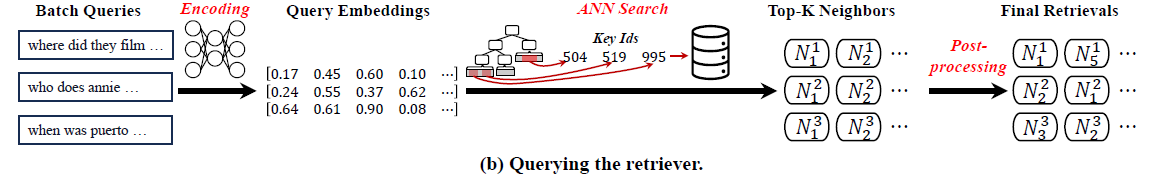
\includegraphics[width=\textwidth]{QueryRetrieverWu2024.png}
        \caption{Vraagafhandeling en ophalen van relevante chunks \cite{Wu2024}}
        \label{fig:RAG bevragen vector database}
    \end{figure}
    
    \paragraph{Generatie}
    
    Zodra de meest relevante informatie is opgehaald, wordt deze gebruikt in het proces. Uiteindelijk blijft het de bedoeling om het LLM-model te bevragen. De opgehaalde documenten worden, samen met de vraag van de gebruiker, toegevoegd aan de context van het model. Hierdoor beschikt het LLM-model over extra informatie en kan het deze verwerken. Dit leidt tot een antwoord voor de gebruiker, gebaseerd op de geïnjecteerde kennis \autocite{Zhao2024}.
    
    \subsection{Cache-Augmented Generation}
    
    Met de opkomst van nieuwe LLM modellen die een grotere context bevatten is het niet altijd nodig om te werken met een RAG architectuur. Wanneer het aantal documenten en de lengte ervan niet dermate groot is kan je ook meteen alle documenten injecteren in de context van een LLM model. Dit zorgt voor een heel simpele en efficiënte benadering om een LLM model bedrijf- of contextspecifieke kennis te geven.
    
    
    \subsection{RAG vs CAG}
    
    
    \subsection{LLM-modellen}
    %TODO opzoeken wat LLM benchmarks zijn en hoe je ze in deze context kan gebruiken
    
    \paragraph{Introductie}
    Om te bepalen welke modellen het meest geschikt zijn voor de ontwikkeling van IT-support chatbot, is een objectieve meetmethode noodzakelijk. Gelukkig bestaan er verschillende platforms die LLM's vergelijken en rangschikken op basis van prestaties. In deze sectie bespreken we enkele van deze platformen en maken we een selectie van modellen die het meest geschikt lijken voor het bouwen van een RAG-model.
    
    %TODO overall dieper ingaan hoe ze te werk gaan als het gaat om vergelijken van een LLM dus de paper lezen en samenvatten wat je ermee kan gaan doen
    
    \paragraph{LiveBench} 
    Een platform dat LLM-modellen evalueert, is LiveBench. Dit platform stelt een rangschikking op voor verschillende modellen en biedt een actuele score bord die elke zes maanden wordt bijgewerkt. Voor deze bachelorproef zal gebruik worden gemaakt van de ranking afkomstig uit november 2024.
    
    LiveBench beoordeelt LLM-modellen op basis van zes categorieën. Binnen elke categorie worden meerdere taken uitgevoerd om een nauwkeurige beoordeling te verkrijgen. De zes categorieën zijn:
    \begin{itemize}
        \item Wiskundige vaardigheden (Math)
        \item Programmeervaardigheden (Coding)
        \item Redeneren en probleemoplossing (Reasoning)
        \item Data-analyse (Data Analysis)
        \item Volgen van instructies (Instruction Following)
        \item Begrip van natuurlijke taal (Language Comprehension)
    \end{itemize}
    
    Elke categorie wordt geëvalueerd op basis van specifieke taken. Dit resulteert uiteindelijk in een algemene rangschikking, waarin zowel de beste modellen per categorie als het beste presterende model overall worden geïdentificeerd.
    
    \begin{figure}[H]
        \centering
        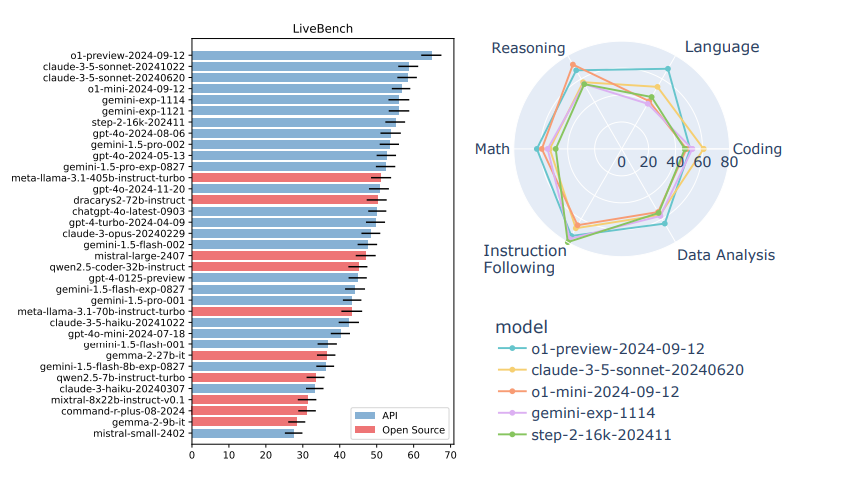
\includegraphics[width=\textwidth]{LiveBenchRanking.png}
        \caption{LiveBench ranking van verschillende LLMs.}
        \label{fig:livebench}
    \end{figure}
    
    Uit de ranking van LiveBench kan geconcludeerd worden dat 3 verschillende organisaties elk een model aanbieden die vanuit globaal oogpunt tot de top 3 behoort. Deze top 3 zijn: 
    \begin{enumerate}
        \item claude-3-5-sonnet-20240620 van Anthropic
        \item Meta-llama-3.1-405b-instruct-turbo van Meta
        \item gpt-4o-2024-05-13 van OpenAI
    \end{enumerate}
    
    \subsubsection{Chatbot arena} 
    
    %TODO uitleggen hoe de scoring werkt van chatbot en eventueel uitleggen wat de verschillen zijn met LiveBench, ik denk vooral dat Chatbot arena getest wordt door mensen en zij hun mening op een grote schaal uitdrukken
    Een andere benchmark tool Chatbot arena, net zoals LiveBench is Chatbot arena een site die een actuele weergave biedt van de beste LLM's op basis van vooraf gedefinieerde categorieën. 
    %Gebruik bronvermelding in plaats van deze manier van schrijven
    Op het moment van het schrijven van deze literatuurstudie is de top 3 LLM's volgens deze site de volgende:
    
    \begin{enumerate}
        \item GPT-4-Turbo van OpenAI
        \item GPT-4-0613 van OpenAI
        \item Mistral-Medium Mistral AI
    \end{enumerate}
    
    Hoewel het doel van beide benchmarks hetzelfde is is de manier van werken wel anders. ChatbotArena gaat gebruikers twee anonieme LLM modellen tegenover elkaar plaatsen, de gebruiker kan vervolgens een eigen vraag stellen en de gebruiker bepaalt zelf welke van de 2 het beste resultaat heeft opgeleverd.
    
    Het voordeel van deze methode is dat de LLM-modellen realistische cases moeten behandelen die door gebruikers zelf worden gesteld. Op basis van resultaten die de LLM modellen tonen kan een gebruiker zijn voorkeur meegeven. Het nadeel van deze manier van werken is dat de gebruikers die deze testen uitvoeren niet respresentatief zijn voor alle gebruikers van LLM-modellen. De gebruikers die deze testen uitvoeren zijn vaak mensen met een interesse in LLM-modellen of mensen die onderzoek doen in dit vakgebied. Desondanks kan op basis van deze stemmen verscheidene modellen tegenover elkaar worden geplaatst. In januari 2024 werden ruim 240.000 stemmen uitgebracht door ongeveer 90.000 gebruikers \autocite{Chiang2024}. 
    
    %TODO zet hier ook de actuele ranking van beide benchmarks. Al was het maar om te duiden dat het een sterk veranderende wereld is waar en dat naar alle waarschijnlijkheid de modellen die nu worden gebruikt waarschijnlijk al achterhaald zullen zijn.
    
    \paragraph{Conclusie}
    
    %TODO Navragen of ze een lijst van criteria hebben welke LLM wel en niet te gebruiken
    Op basis van de 2 benchmarks die hier werden besproken kan niet meteen éénduidig besloten worden welke modellen het best zouden gebruikt worden voor het maken van het RAG model. Aangezien dit een zeer volatiele omgeving is met veel en snelle ontwikkelingen zijn de modellen die vandaag het beste scoren over een maand potentieel voorbij gestoken door nieuwe modellen. Desalniettemin bevatten deze benchmarks heel wat nuttige informatie en inzichten over de sterktes van bepaalde modellen tegenover andere modellen. 
    

\section{De AI Act en de belangrijkste richtlijnen}
Wat houdt de AI Act in, en wat zijn de belangrijkste richtlijnen die hierin moeten worden gevolgd?

\section{Best practices voor IT-supportprocessen}
Wat zijn de bestaande best practices voor de organisatie van IT-supportprocessen?
